\chapter{Results}
\label{chapter:results}

% After covering XBRL, the Brel API and its implementation, we can now evaluate Brel against the requirements that we defined in section \ref{sec:goals}.
% We will evaluate Brel based on correctness first and performance second.
% This chapter will also cover Brel's robustness and usability in a qualitative manner.

% The usability of Brel will be evaluated by using it to implement a simple CLI XBRL report viewer.
% It will cover every feature of the Brel API and serve as a proof of concept for the Brel API.

% Even though Brel's performance is not part of the requirements set by this thesis,
% it still serves as an important metric.
% It will enable future versions of Brel to compare their performance against this initial version of Brel.

% For testing Brel's correctness, we will use XBRL conformance suites.
% Additionally, we will look at the at a hand-picked XBRL report and compare the structure that Brel extracts
% from it against the results that the XBRL viewer Arelle produces.
% This serves as a qualitative measure of correctness.

% Robustness is a qualitative metric that is hard to measure.
% We will evaluate Brel's robustness by loading the 8K and 10Q reports of the 30 largest US companies by market capitalization at the time of writing.
% This will give us a good idea of how robust Brel is in practice.

Following the discussion on XBRL, the Brel API, and its implementation, 
we are now in a position to assess Brel in light of the objectives outlined in section \ref{sec:goals}. 
The evaluation will prioritize usability, correctness, robustness and performance.
% Additionally, this chapter will qualitatively discuss Brel's robustness and usability.

The usability of Brel will be assessed through the development of a simple CLI tool for viewing XBRL reports. 
This tool will demonstrate the capabilities of the Brel API and act as a practical example of its application.

The assessment of Brel's correctness will involve the use of an XBRL conformance suite. 
Furthermore, we will conduct an analysis of a selected component of an XBRL report, 
comparing the structure Brel extracts with that produced by the XBRL viewer Arelle. 
This comparison will offer a qualitative evaluation of Brel's accuracy.

Robustness, being a qualitative metric, presents challenges in measurement. 
However, by loading the 10K and 10Q reports of the 50 largest US companies by market capitalization as of the date of this analysis, 
we can gain valuable insights into Brel's practical robustness.

Although this thesis does not explicitly list Brel's performance as a requirement, 
it remains a crucial aspect of the evaluation. 
Assessing Brel's performance will provide a benchmark for future versions of the software, 
facilitating performance comparisons over time.

\section{Usability}
\label{sec:usability}

% One of the goals of this thesis is to create a usable API for working with XBRL reports.
% To evaluate the usability of the Brel API, we will implement a simple CLI XBRL report viewer.
% This viewer will cover every feature of the Brel API and serve as a proof of concept for the Brel API.

% The CLI XBRL report viewer will be implemented in Python and will use the Brel API to load and display XBRL reports.
% It will be able to load XBRL reports from local files and from URLs.

% The viewer will be able to display the following information about an XBRL report:
A primary aim of this thesis is to develop a user-friendly API for XBRL report processing.  
For assessing the Brel API's usability, a basic Command Line Interface (CLI) XBRL report viewer will be created.  
This viewer will showcase a subset of all features of the Brel API, demonstrating its practicality.

The CLI XBRL report viewer, coded in Python, will employ the Brel API for XBRL report management.  
It will have the capability to access XBRL reports both locally and via URLs.
The viewer is available as an example in the Brel repository\cite{brel_source}.

Regarding an XBRL report, the viewer will present various types of information:

\begin{itemize}
    \item The facts in the report, which can be filtered by concept and a dimension.\footnote{Filters for entity, period, and unit are not implemented since most reports have very few entities, periods, and units.}
    % For each fact, the viewer should display all characteristics of the fact in a easy-to-read manner.
    For each fact, the viewer displays all characteristics in a human-readable format.
    \item The components of a report together with their networks.
    % The viewer should be able to display the relationships between report elements in the networks in a human-readable manner.
    The viewer presents the relationships between report elements in the networks in a human-readable format.
\end{itemize}

Before implementing the viewer, we will first install Brel and its dependencies.
Since Brel is published on the Python Package Index (PyPI), we can install it using pip.

\begin{lstlisting}[language=bash]
pip install brel-xbrl
\end{lstlisting}

After installing Brel, we can start implementing the viewer.
The viewer will be implemented in a single file called \texttt{viewer.py}.
The first part of the implementation is shown in figure \ref{fig:viewer_1}.
It shows the imports and the command-line interface (CLI) definition of the viewer.

\begin{figure}[H]
    \centering
    \lstinputlisting[
        language=Python, 
        basicstyle=\scriptsize\ttfamily,
        firstline=1, lastline = 8
    ]{../../examples/cli.py}
    \caption{The implementation of the CLI XBRL report viewer responsible for the CLI.}
    \label{fig:viewer_1}
\end{figure}


The viewer is implemented as a command-line interface (CLI) using the \texttt{argparse} module.
It has two subcommands: \texttt{facts} and \texttt{components}.
The former subcommand is used to display the facts in an XBRL report, 
% and the \texttt{components} subcommand is used to display the components of a report together with their networks.
whereas the latter subcommand is used to display the components together with their networks.
Both subcommands take a single argument, which acts as a filter for the facts and components that are displayed.

% The facts filter is used to filter the facts in the report by concept or dimension.
% If a fact has the concept or dimension that matches the filter, it will be displayed.
% The components filter is used to filter the components in the report by URI.
% If a component has a URI that contains the filter as a substring, it will be displayed
% \footnote{We use a substring since typing out the full URI of a component can be cumbersome.}.
The report's facts filter selects facts based on matching concepts or dimensions.
A fact is displayed if it aligns with the filter's specified concept or dimension.
The components filter operates by screening report components via their URI.
A component is shown if its URI includes the filter's substring\footnote{Substrings are used to simplify the process, as typing the full URI can be cumbersome.}.

% First of all, the viewer uses \texttt{Filing.open} on line 11 to open the XBRL report.
% The argument of this method can be a local file path or a URI.
% Since Brel potentially needs to download the report from the internet, the call to \texttt{Filing.open} can take a few seconds to complete.
% The figure \ref{fig:viewer_2} shows the second part of the implementation of the viewer responsible for loading the report.
Initially, the viewer employs \texttt{Filing.open} to load the XBRL report.
This method's argument can be either a local file path or a URI.
Due to the potential need for Brel to download the report, executing \texttt{Filing.open} might take a few seconds.
The following figure illustrates the viewer's second part, focusing on the report's loading process.

\begin{figure}[H]
    \centering
    % \caption{The implementation of the XBRL report viewer responsible for loading the report}
    \lstinputlisting[
        language=Python, 
        basicstyle=\scriptsize\ttfamily,
        firstline=11, lastline = 12
    ]{../../examples/cli.py}
    \label{fig:viewer_2}
    \caption{The implementation of the CLI XBRL report viewer responsible for loading the report.}
\end{figure}

% The facts portion of the viewer \ref{fig:viewer}, which ranges from lines 12 to 23, uses the Brel methods \texttt{report.get\_all\_facts}, 
% \texttt{fact.get\_concept}, \texttt{fact.get\_aspects}, and \texttt{utils.pprint}.
% Some of the methods were not covered in chapter \ref{chapter:api} since they are merely convenience methods that are not part of the core API.
% For example, \texttt{fact.get\_concept} is an alias of \texttt{fact.get\_characteristic(Aspect.CONCEPT)}.
% Furthermore, the \texttt{utils.pprint} method is a convenience method that pretty-prints most Brel objects in a human-readable manner.
% It simply calls both \texttt{fact.get\_aspects} and \texttt{fact.get\_characteristic} for each fact and pretty-prints the result.
The next section of the implementation deals with the facts portion of the viewer.
First, it gets all facts in the report.
Then, it filters the facts that either have the concept or dimension that matches the filter.
Next, it pretty-prints the facts in a human-readable manner.
We can get all facts in the report using the method \texttt{report.get\_all\_facts}.
The \texttt{fact.get\_concept} and \texttt{fact.get\_aspects} methods can be used to get the concept and aspects of each fact.
Since dimensions are just aspects, we can check all aspects of a fact to see if one of them matches the filter.
Finally, we can use the \texttt{utils.pprint} method to pretty-print the facts in a human-readable manner.
\texttt{utils.pprint} is a convenience method that, given a list of facts, it calls both \texttt{fact.get\_aspects} and \texttt{fact.get\_characteristic} for each fact and pretty-prints the result.
Figure \ref{fig:viewer_3} shows the third part of the implementation of the viewer responsible for displaying the facts in the report.

\begin{figure}[H]
    \centering
    % \caption{The implementation of the XBRL report viewer responsible for displaying the facts in the report}
    \lstinputlisting[
        language=Python, 
        basicstyle=\scriptsize\ttfamily,
        firstline=13, lastline = 21
    ]{../../examples/cli.py}
    \caption{The implementation of the CLI XBRL report viewer responsible for displaying facts.}
    \label{fig:viewer_3}
\end{figure}

% The components portion of the viewer should be implemented in a similar manner.
% First, it should get all components in the report using \texttt{report.get\_all\_components}.
% Then, it should filter the components that have a URI that contains the filter as a substring.
% This is done using the \texttt{component.get\_uri} method.
% Finally, it should pretty-print the components in a human-readable manner using \texttt{utils.pprint}.
% The method \texttt{utils.pprint} not only works for lists of facts, but also for a list components.
% For each network in the component, the \texttt{utils.pprint} uses a DFS algorithm on both the
% \texttt{network.get\_roots} and \texttt{network\_node.get\_children} methods to pretty-print the network in a human-readable manner.
% It also automatically uses the labels of report elements if they are available.
% The figure \ref{fig:viewer_4} shows the fourth and final part of the implementation of the viewer responsible for displaying the components in the report.
% The viewer's components section should be implemented following a similar approach.  
The viewer's components section is implemented in a similar manner.
Initially, it needs to retrieve all components in the report by using \texttt{report.get\_all\_components}.  
Next, it filters those components whose URI contains the specified substring, utilizing \texttt{component.get\_uri} for this purpose.  
Finally, \texttt{utils.pprint} is used to format the components in a human-readable manner.
The \texttt{utils.pprint} method is versatile, functioning with both fact lists and component lists.  
For each network within a component, \texttt{utils.pprint} employs a Depth-First Search (DFS) algorithm,  
applying it to both \texttt{network.get\_roots} and \texttt{network\_node.get\_children} to format the network clearly and coherently.  
This method also automatically incorporates the labels of report elements when available.  
Figure \ref{fig:viewer_4} displays the final part of the viewer's implementation, focusing on presenting the report's components.


\begin{figure}[H]
    \centering
    % \caption{The implementation of the XBRL report viewer responsible for displaying the components in the report}
    \lstinputlisting[
        language=Python, 
        basicstyle=\scriptsize\ttfamily,
        firstline=22, lastline = 34
    ]{../../examples/cli.py}
    \caption{The implementation of the CLI XBRL report viewer}
    \label{fig:viewer_4}
\end{figure}

The implementation of the viewer is now complete.
The viewer can be used to display the facts and components of an XBRL report using only a few lines of code and using python's built-in list comprehension.

% As shown in figure \ref{fig:viewer}, filtering the facts in a report can be done using only a few lines of code and using python's built-in list comprehension.
% The method \texttt{report.get\_all\_facts} is used to get all facts in the report, 
% where the methods \texttt{fact.get\_concept} and \texttt{fact.get\_aspects} are used to get the concept and aspects of each fact and filter accordingly.

% The components portion of the viewer \ref{fig:viewer}, which ranges from lines 24 to 34,
% uses the Brel methods \texttt{report.get\_all\_components}, \texttt{component.get\_uri} and \texttt{utils.pprint}.
% The \texttt{utils.pprint} not only works for lists of facts, but also for a list components.
% For each network in the component, the \texttt{utils.pprint} uses a DFS algorithm on both the
% \texttt{network.get\_roots} and \texttt{network\_node.get\_children} methods to pretty-print the network in a human-readable manner.
% It also automatically uses the labels of report elements if they are available.
% Similar to the facts portion, the \texttt{get\_all\_components} method is used to get all components in the report,
% where the \texttt{component.get\_uri} method is used to get the URI of each component and filter accordingly.

% Again, as shown in figure \ref{fig:viewer}, filtering the components in a report can be done using only a few lines of code and using python's built-in list comprehension.


% For instance, the command \texttt{python viewer.py facts us-gaap:Revenue} will display all facts in the report that have the concept \texttt{us-gaap:Revenue}.
% The command \texttt{python viewer.py components CoverPage} will display all components that have the substring \texttt{CoverPage} in their URI.
% \begin{lstlisting}[language=Python, caption={The implementation of the CLI XBRL report viewer}, label={lst:viewer}]

The following two examples illustrate how the viewer can be used to display the facts and components of an XBRL report.
Each example will show both the command that is used to display the information and the output of the command.
For both examples, we will use the Q3 2023 10-Q report of Apple Inc. (AAPL) that is available on the SEC's website\cite{aapl_10q_2023_q3}.
% For brevity, we have downloaded the report and saved in an archive called \texttt{report.zip}.
To keep the commands simple, we will use the \texttt{report.zip} file that contains the report.
However, the viewer can also load reports from URLs.

\begin{figure}[H]
    \centering
    \begin{lstlisting}[language=bash]
python viewer.py report.zip --facts us-gaap:Assets
\end{lstlisting}
    % make font tiny and use monospaced font
    \begin{lstlisting}[language=bash, basicstyle=\scriptsize\ttfamily]
--------------------------------------------------------------------------------------------+
|                                    Facts Table                                            |
+----------------+---------------+------------------------------------+------+--------------+
|        concept |        period |                             entity | unit |        value |
+----------------+---------------+------------------------------------+------+--------------+
| us-gaap:Assets | on 2023-07-01 | {http://www.sec.gov/CIK}0000320193 |  usd | 335038000000 |
| us-gaap:Assets | on 2022-09-24 | {http://www.sec.gov/CIK}0000320193 |  usd | 352755000000 |
+----------------+---------------+------------------------------------+------+--------------+
\end{lstlisting}
    \caption{Assets in the Q3 2023 10-Q report of Apple Inc.}
    \label{fig:aapl_assets}
\end{figure}

As shown in figure \ref{fig:aapl_assets}, the command returns the facts in the report that have the concept \texttt{us-gaap:Assets}.
It clearly shows the concept, period, entity, unit, and value for both facts.
Neither fact has additional dimensions.

\begin{figure}[H]
    \begin{lstlisting}[language=bash]
python viewer.py report.zip --components InsiderTradingArrangements
\end{lstlisting}
    % make font tiny and use monospaced font. allow non-utf8 characters
    \begin{lstlisting}[basicstyle=\scriptsize\ttfamily, language=bash, extendedchars=true, escapeinside={\<}{\>}]
Component: http://xbrl.sec.gov/ecd/role/InsiderTradingArrangements
Info: 995445 - Disclosure - Insider Trading Arrangements
Networks: 
link role: .../InsiderTradingArrangements, link name: link:presentationLink
arc roles: ['.../parent-child'], arc name: link:presentationArc
└──[LINE ITEMS] Insider Trading Arrangements [Line Items]
    ├──[HYPERCUBE] Trading Arrangements, by Individual [Table]
    │  ├──[DIMENSION] Trading Arrangement [Axis]
    │  │  └──[MEMBER] All Trading Arrangements [Member]
    │  └──[DIMENSION] Individual [Axis]
    │     └──[MEMBER] All Individuals [Member]
    ├──[CONCEPT] Material Terms of Trading Arrangement [Text Block]
    │   ...
    └──[CONCEPT] Trading Arrangement, Securities Aggregate Available Amount
\end{lstlisting}
\caption{Insider trading arrangements in the Q3 2023 10-Q report of Apple Inc. The output is truncated.}

\label{fig:aapl_insider_trading}
\end{figure}

% As shown in figure \ref{fig:aapl_insider_trading}, 
% the command returns the component identified with URI \texttt{http://xbrl.sec.gov/ecd/role/InsiderTradingArrangements}.
% It clearly shows the URI, label, and networks for the component.
% The networks are pretty-printed in a human-readable manner and 
% show the relationships between report elements in the networks.
% Additionally, the network shows the link/arc roles and names for each network, which can be useful for debugging.

% This example shows that the Brel API is easy to use and can be used to implement a simple CLI XBRL report viewer.
% The viewer is able to display the facts and components using only a few lines of code and using python's built-in list comprehension.
% This section does not cover every feature of the Brel API, but it serves as a proof of concept.
% More examples are available both in the Brel documentation\cite{brel_api} and in the Brel repository\cite{brel_source}.

As depicted in figure \ref{fig:aapl_insider_trading},  
the command retrieves the component with the URI \texttt{http://xbrl.sec.gov/ecd/role/InsiderTradingArrangements}.  
Figure \ref{fig:aapl_insider_trading} shows the URI, label, and networks associated with the component.  
These networks are formatted in a user-friendly manner,  
illustrating the connections between various report elements within the networks.  
Furthermore, each network includes the link/arc roles and names, providing valuable insights for debugging purposes.

This example demonstrates the user-friendliness and practical utility of the Brel API.  
It exemplifies how a simple Command Line Interface (CLI) XBRL report viewer can be implemented using the Brel API.  
The viewer efficiently displays facts and components with minimal coding, leveraging Python's built-in list comprehension.  
While this section does not explore all features of the Brel API, it effectively serves as a proof of concept.  
For additional examples and in-depth understanding, readers can refer to the Brel documentation\cite{brel_api} and the Brel source code repository\cite{brel_source}.

% \end{lstlisting}

\section{Correctness}
\label{sec:correctness}

To evaluate Brel's correctness, we will use Charles Hoffman's XBRL conformance suite \cite{hoffman_conformance_suite}.
The conformance suite contains a set of XBRL reports that are known to be correct.
It checks for conformance to the XBRL specification from both a syntactic and a logical point of view.
Brel will ignore the logical checks, as it only deals with the syntactic part of the XBRL specification.

We will not cover either the SEC's or the ESMA's conformance suites, 
as they contain many test cases that are not relevant to Brel in its current state.

Besides the conformance suite, we will also look at a hand-picked XBRL report.
Since the source files of an XBRL report are not human-readable, 
we will use the XBRL platform Arelle\cite{arelle} to visualize the structures that Brel extracts from the reports.
% We will compare the structures that Brel extracts from them against the structures that the XBRL specification prescribes.
Arelle closely follows the XBRL specification and can therefore be considered a reliable source of truth.
We will compare the structures that Brel extracts from the reports against the structures that Arelle extracts from the same reports.
For the sake of brevity, we will only look at a single network within the report.
Even though this evaluation only covers a single component within the report,
it will give us a more intuitive understanding of Brel's correctness compared to the conformance suite.
Brel also contains its own test suite, which is not covered in this thesis.

\subsection{Conformance suite}

Charles Hoffman maintains a conformance suite for XBRL \cite{hoffman_conformance_suite}.
It covers both the syntactic and the semantic aspects of the XBRL specification.
The conformance suite contains a set of XBRL reports that are known to be correct or incorrect.
It checks for conformance to the XBRL specification from both a syntactic and a logical point of view.

Since Brel only deals with the syntactic part of the XBRL specification, 
it will be unable to check the logical part of the conformance suite.
Therefore reports that are syntactically correct, but semantically incorrect, will be considered correct by Brel.

Figure \ref{fig:conformance_suite} shows the results of running the conformance suite on Brel.

\begin{figure}[H]
  \centering
  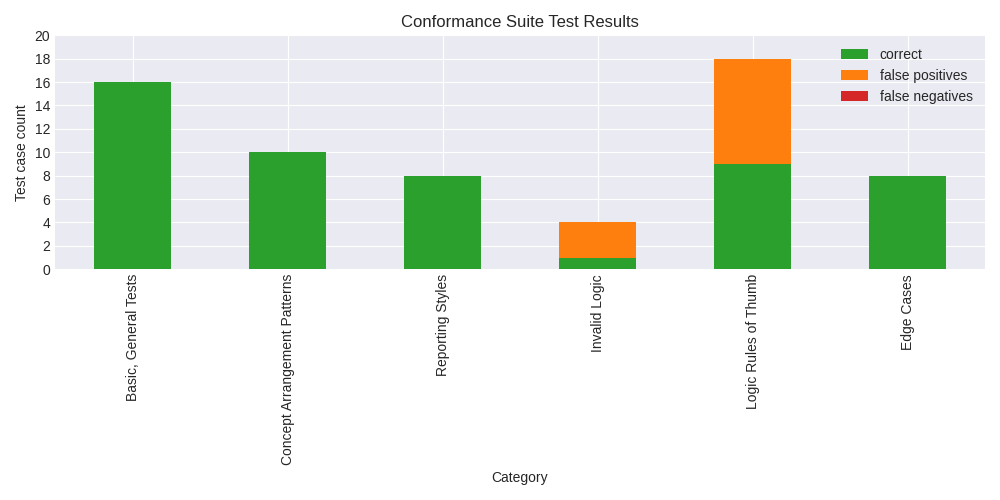
\includegraphics[width=1\textwidth]{images/seattle_method_test_results.png}
    \caption{Conformance suite results}
    \label{fig:conformance_suite}
\end{figure}

The conformance suite contains 77 test cases, of which 22 are considered logical checks.
Of the 22 logical checks, Brel passes 10 and fails 12.
Since Brel only deals with the syntactic part of the XBRL specification,
the test cases it passed it passed by coincidence.
We still list the results for completeness.

Of the 55 syntactic checks, Brel passes all of them.
This is a good result, as it shows that Brel is able to parse XBRL reports correctly.
However, it is important to note that the conformance suite is not exhaustive.
Also, conformance suite test cases are not necessarily representative of real-world XBRL reports.
They serve as a good starting point, but they are not enough to guarantee Brel's correctness.

\subsection{Hand-picked XBRL reports}

We will also look at a hand-picked XBRL report.
We will compare the structures that Brel extracts from them against the structures that the XBRL specification prescribes.
Since the source files of an XBRL report meant to be read by machines,
we will use the XBRL platform Arelle to visualize the structures that Brel extracts from the reports.
Arelle is a mature, robust and widely used XBRL platform and can therefore be considered a reliable source of truth.
It closely follows the XBRL specification, including the OIM.

% The hand-picked XBRL reports are:

% A report from the SEC's EDGAR database \cite{sec_edgar}. 
The hand picked report is from the SEC's EDGAR database \cite{sec_edgar}.
In this case we will use Microsoft's 10K report for the fiscal year 2022.
\footnote{Available at \url{https://www.sec.gov/ixviewer/ix.html?doc=/Archives/edgar/data/789019/000095017023035122/msft-20230630.htm}}
This report will be loaded directly from the EDGAR database by providing the URL of the report to Brel.
% A report from the ESMA's ESEF database hosted by the XBRL Foundation\cite{esma_database}.
% In this case we will use Novo Nordisk's 2023 financial report covering the first three quarters of 2023.
% \footnote{Available at \url{https://filings.xbrl.org/filing/549300DAQ1CVT6CXN342-2023-09-30-ESEF-DK-0}}
% This report will be loaded from disk.

% We will look at the \texttt{DocumentAndEntityInformation} component and all facts associated with the concepts within its presentation network.
% It acts as a cover page for the report and contains information about the company, the report, and the auditor.
% Its presentation network is a good starting point, since the information in it is understandable by non-accountants.
% Furthermore, Brel employs the same network parsing algorithm for all networks, so the results of this evaluation will be representative of Brel's correctness.
We will look at the \texttt{ComprehenisveIncomeStatement} component and all facts associated with the concepts within its presentation network.
Its presentation network acts as a good sanity check, since the information in it is understandable by non-accountants.
Furthermore, Brel employs the same network parsing algorithm for all networks, so the results of this evaluation will be representative of Brel's correctness.

% The following sections show the results of the evaluation.
% The report is loaded directly from the EDGAR database by providing the URL of the report to Brel.
% First, let us look at the cover page as it is presented in Arelle.
First, let us look at the comprehensive income statement as it is presented in Arelle.

\begin{figure}[H]
  \centering
%   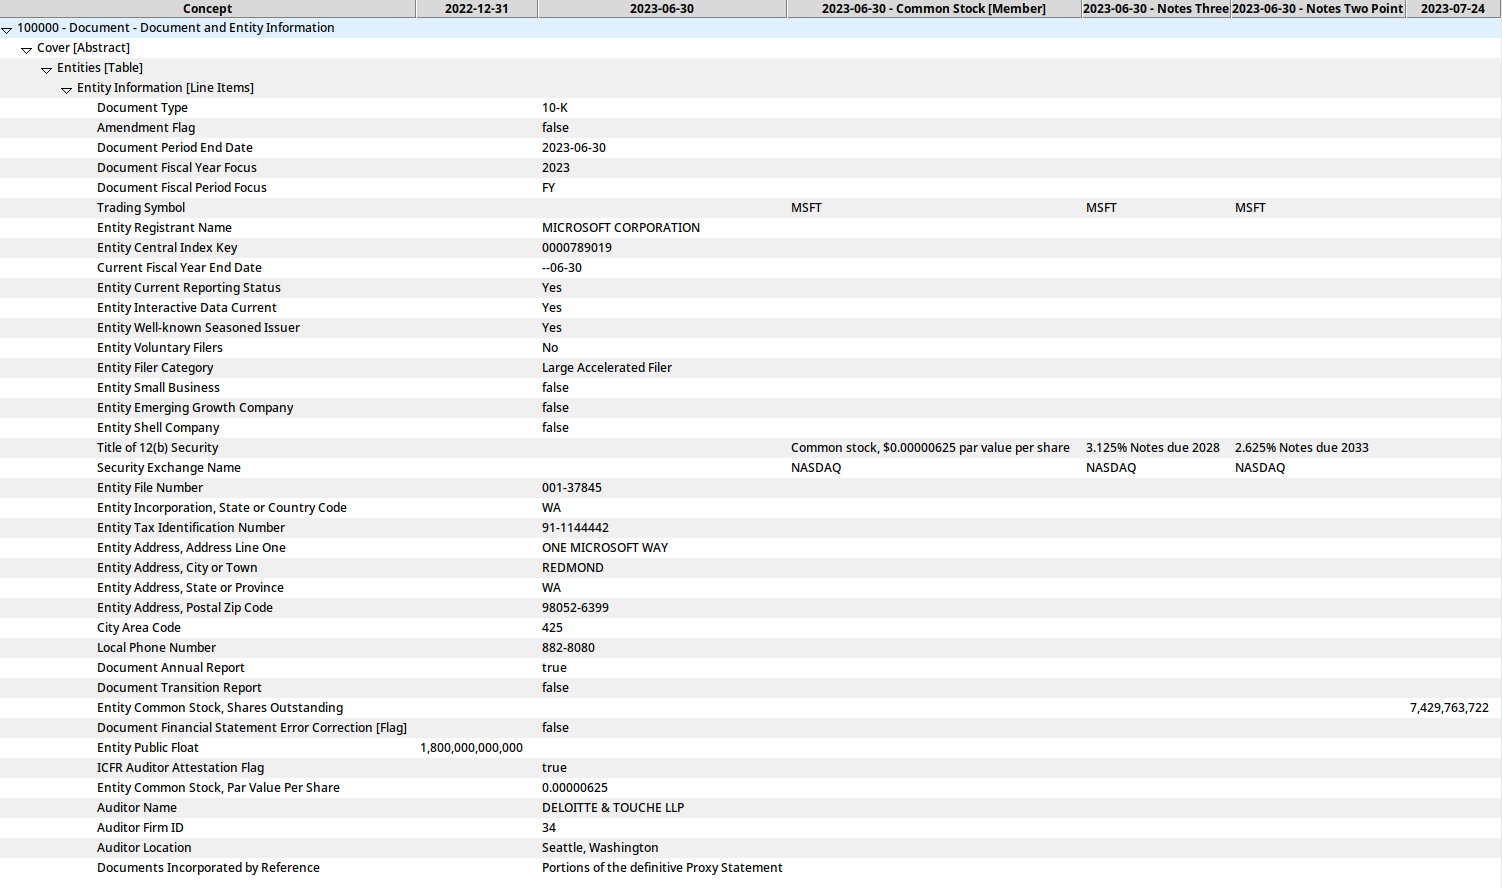
\includegraphics[width=1\textwidth]{images/msft_coverpage_arelle.png}
    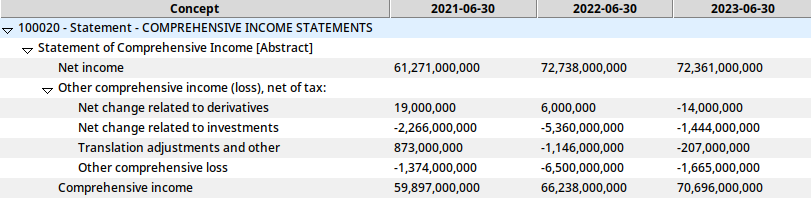
\includegraphics[width=1\textwidth]{images/msft_income_statement_arelle.png}
    \caption{Microsoft's 10K report cover page in Arelle}
    \label{fig:msft_income_statement_arelle}
\end{figure}

% The figure \ref{fig:msft_coverpage_arelle} shows the cover page of Microsoft's 10K report in Arelle.
The figure \ref{fig:msft_income_statement_arelle} shows the comprehensive income statement of Microsoft's 10K report in Arelle.
Brel works different from Arelle, as it does not visualize the network and its facts in a graphical manner.
However, using the \texttt{viewer.py} script we have written in section \ref{sec:usability}, 
we can visualize the cover page in a textual manner.
The figure \ref{fig:msft_income_statement_network} shows the hierarchy of cover page of Microsoft's 10K report in Brel.

\begin{figure}[H]
    \begin{lstlisting}[basicstyle=\small\ttfamily]
Component: .../Role_StatementCOMPREHENSIVEINCOMESTATEMENTS
Info: 100020 - Statement - COMPREHENSIVE INCOME STATEMENTS

link name: link:presentationLink
arc roles: ['.../parent-child'], arc name: link:presentationArc
└──[ABSTRACT] Statement of Comprehensive Income [Abstract]
    ├──[CONCEPT] Net Income (Loss)
    ├──[ABSTRACT] Other comprehensive income (loss), net of tax:
    │  ├──[CONCEPT] Net change related to derivatives
    │  ├──[CONCEPT] Net change related to investments
    │  ├──[CONCEPT] Translation adjustments and other
    │  └──[CONCEPT] Other comprehensive income (loss)
    └──[CONCEPT] Comprehensive Income (Loss), Net of Tax, Attributable to Parent
    \end{lstlisting}
    \caption{Microsoft's 10K presentation network in Brel}
    \label{fig:msft_income_statement_network}
\end{figure}

The figure \ref{fig:msft_income_statement_network} shows the hierarchy of the comprehensive income statement of Microsoft's 10K report in Brel.
Note that the labels between the two figures are different, since Arelle might use different label roles from the ones used in Brel.
The only difference between the content of the two figures is the fact that Arelle includes the facts associated with the concepts in the network, 
while Brel only includes the report elements and their relationships.

Luckily, we can use the \texttt{viewer.py} and filter all facts that have concepts present in figure \ref{fig:msft_income_statement_network}
to visualize the facts associated with the concepts in the network.
The output of the \texttt{viewer.py} script is shown in figure \ref{fig:msft_income_statement_facts}.
Note that the output has been truncated.
Also note that XBRL reports can contain duplicate facts, as they can be reported in different contexts.
Arelle does not show duplicate facts, while Brel does.

\begin{figure}[H]
  \begin{lstlisting}[basicstyle=\tiny\ttfamily]
+-------------------------------------------------------------------------------------------------------------------------+
| Facts Table                                                                                                             |
+------------------------------------------------------+-------------------------------+------------+-------+-------------+
|                                              concept |                        period |     entity |  unit |       value |
+------------------------------------------------------+-------------------------------+------------+-------+-------------+
|                                us-gaap:NetIncomeLoss | from 2020-07-01 to 2021-06-30 | 0000789019 |  USD  | 61271000000 |
|                                us-gaap:NetIncomeLoss | from 2021-07-01 to 2022-06-30 | 0000789019 |  USD  | 72738000000 |
|                                us-gaap:NetIncomeLoss | from 2022-07-01 to 2023-06-30 | 0000789019 |  USD  | 72361000000 |
|           us-gaap:OtherComprehensiveIncomeLossCas... | from 2020-07-01 to 2021-06-30 | 0000789019 |  USD  |    19000000 |
|           us-gaap:OtherComprehensiveIncomeLossCas... | from 2021-07-01 to 2022-06-30 | 0000789019 |  USD  |     6000000 |
|           us-gaap:OtherComprehensiveIncomeLossCas... | from 2022-07-01 to 2023-06-30 | 0000789019 |  USD  |   -14000000 |
|               us-gaap:OtherComprehensiveIncomeLos... | from 2020-07-01 to 2021-06-30 | 0000789019 |  USD  | -2266000000 |
|               us-gaap:OtherComprehensiveIncomeLos... | from 2021-07-01 to 2022-06-30 | 0000789019 |  USD  | -5360000000 |
|               us-gaap:OtherComprehensiveIncomeLos... | from 2022-07-01 to 2023-06-30 | 0000789019 |  USD  | -1444000000 |
| us-gaap:OtherComprehensiveIncomeLossForeignCurren... | from 2020-07-01 to 2021-06-30 | 0000789019 |  USD  |   873000000 |
| us-gaap:OtherComprehensiveIncomeLossForeignCurren... | from 2021-07-01 to 2022-06-30 | 0000789019 |  USD  | -1146000000 |
| us-gaap:OtherComprehensiveIncomeLossForeignCurren... | from 2022-07-01 to 2023-06-30 | 0000789019 |  USD  |  -207000000 |
|                        us-gaap:OtherComprehensive... | from 2020-07-01 to 2021-06-30 | 0000789019 |  USD  | -1374000000 |
|                        us-gaap:OtherComprehensive... | from 2021-07-01 to 2022-06-30 | 0000789019 |  USD  | -6500000000 |
|                        us-gaap:OtherComprehensive... | from 2022-07-01 to 2023-06-30 | 0000789019 |  USD  | -1665000000 |
|                  us-gaap:ComprehensiveIncomeNetOfTax | from 2020-07-01 to 2021-06-30 | 0000789019 |  USD  | 59897000000 |
|                  us-gaap:ComprehensiveIncomeNetOfTax | from 2021-07-01 to 2022-06-30 | 0000789019 |  USD  | 66238000000 |
|                  us-gaap:ComprehensiveIncomeNetOfTax | from 2022-07-01 to 2023-06-30 | 0000789019 |  USD  | 70696000000 |
+------------------------------------------------------+-------------------------------+------------+-------+-------------+
    \end{lstlisting}
    \caption{Microsoft's 10K facts in Brel}
    \label{fig:msft_income_statement_facts}
\end{figure}

The figure \ref{fig:msft_income_statement_facts} clearly shows that Brel is able to extract the facts from the comprehensive income statement of Microsoft's 10K report correctly.
All facts present in figure \ref{fig:msft_income_statement_arelle} are also present in figure \ref{fig:msft_income_statement_facts} and vice versa.
Each individual fact is also correct, as it is associated with the correct concept, period, entity, unit, and value.
Brel represents these characteristics differently from Arelle.
For example, Arelle visualizes concepts using their labels, while Brel visualizes concepts using their QNames.
However, the values themselves represent the same information.
The only difference is between the representation of the facts, as Arelle visualizes the facts as a table, where the rows are the concepts and the columns are the periods.
Brel visualizes the facts as a table representing a hypercube.

We can conclude that Brel is able to extract the structures from the comprehensive income statement of Microsoft's 10K report correctly.
This is a good result, as it shows that Brel is able to parse XBRL reports correctly.
However, it is important to note that this evaluation only covers a single component within the report.
It does not cover the full range of Brel's functionality or its correctness.
This example serves as a vertical slice of Brel's correctness.
Together with the conformance suite, it gives us a good idea of Brel's correctness.


\section{Robustness}
\label{sec:robustness}

Brel's robustness against real-world XBRL reports is paramount to its usefulness.
Therefore, we will evaluate Brel's robustness by loading the 10K and 10Q reports of the 30 largest US companies by market capitalization at the time of writing
\footnote{Time of writing: 29 January 2024}.
The list of companies that we will use is shown in table \ref{table:companies}.
% This list was generated by using the list of the 100 largest US companies by market capitalization\cite{largest_us_companies} and removing all companies that do not have any 10K or 10Q reports.
This list was generated by cropping the list of the 100 largest US companies by market capitalization\cite{largest_us_companies}.
We limited the list to US companies since the SEC mandates that all US companies must file their financial reports in XBRL\cite{sec_ixbrl}.

% "Rank","Name","Symbol","marketcap","price (USD)","country"
% "1","Microsoft","MSFT","3009100644352","403.93","United States"
% "2","Apple","AAPL","2975178948608","192.42","United States"
% "3","Alphabet (Google)","GOOG","1913839550464","153.79","United States"
% "4","Amazon","AMZN","1644346081280","159.12","United States"
% "5","NVIDIA","NVDA","1507465756672","610.31","United States"
% "6","Meta Platforms (Facebook)","META","1012884701184","394.14","United States"
% "7","Berkshire Hathaway","BRK-B","837177376768","385.4","United States"
% "8","Eli Lilly","LLY","606844485632","639.25","United States"
% "9","Tesla","TSLA","582537052160","183.25","United States"
% "10","Broadcom","AVGO","564053737472","1204.88","United States"
% "11","Visa","V","542508843008","267.94","United States"
% "12","JPMorgan Chase","JPM","495597846528","172.28","United States"
% "13","UnitedHealth","UNH","465422254080","503.2","United States"
% "14","Walmart","WMT","442252623872","164.27","United States"
% "15","Exxon Mobil","XOM","411667300352","103","United States"
% "16","Mastercard","MA","411242921984","438.53","United States"
% "17","Johnson & Johnson","JNJ","383961169920","159.5","United States"
% "18","Procter & Gamble","PG","367400517632","156.14","United States"
% "19","Home Depot","HD","353616592896","355.3","United States"
% "20","Oracle","ORCL","316125544448","114.64","United States"
% "21","Merck","MRK","306160304128","120.82","United States"
% "22","Costco","COST","304787881984","686.88","United States"
% "23","AbbVie","ABBV","290254749696","164.4","United States"
% "24","AMD","AMD","286347395072","177.25","United States"
% "25","Chevron","CVX","281539051520","149.14","United States"
% "26","Adobe","ADBE","277496365056","613.93","United States"
% "27","Salesforce","CRM","270981922816","279.94","United States"
% "28","Bank of America","BAC","263945224192","33.43","United States"
% "29","Coca-Cola","KO","256680837120","59.37","United States"
% "30","Netflix","NFLX","249661423616","570.42","United States"

% make a 3x10 table instead that contains just the names of the companies
\begin{table}[H]
    \centering
    % make the text scriptsize
    % \scriptsize
    \begin{tabular}{|l l l|}
        \hline
        Microsoft & Apple & Alphabet (Google) \\
        Amazon & NVIDIA & Meta Platforms (Facebook) \\
        Berkshire Hathaway & Eli Lilly & Tesla \\
        Broadcom & Visa & JPMorgan Chase \\
        UnitedHealth & Walmart & Exxon Mobil \\
        Mastercard & Johnson \& Johnson & Procter \& Gamble \\
        Home Depot & Oracle & Merck \\
        Costco & AbbVie & AMD \\
        Chevron & Adobe & Salesforce \\
        Bank of America & Coca-Cola & Netflix \\
        \hline
    \end{tabular}
    \caption{The 30 largest US companies by market capitalization at the time of writing}
    \label{table:companies}
\end{table}

The table \ref{table:companies} shows the companies that we will use to evaluate Brel's robustness.
The table shows the largest three companies in the first row from left to right, followed by the next three companies in the second row, and so on.
For all companies, we will use the latest five 10K and 10Q reports that are available on the EDGAR database\cite{sec_edgar}.
We will load the reports using the Brel API and check for one of three outcomes:

\begin{enumerate}
    \item The report is loaded successfully without any errors.
    \item The report is loaded successfully, but Brel logs a warning or an error.
    \item Brel raises an exception while loading the report.
\end{enumerate}

Since Brel loads reports eagerly, we will only load the reports and not perform any operations on them.
This will give us a good idea of how robust Brel is in practice.
However, it does not cover the full range of Brel's functionality or its correctness.
This functionality was already covered in section \ref{sec:correctness}.
The results of the robustness evaluation are shown in table \ref{table:robustness}.


\section{Performance}
\label{sec:performance}

% The performance of Brel is an important aspect of its evaluation.
% This section will evaluate Brel's performance by measuring the time it takes to load and extract data from XBRL reports.
% The performance of Brel is not part of the requirements set by this thesis.
% However, it serves as an important metric for future versions of Brel to compare their performance against this initial version of Brel.
Assessing Brel's performance is a key part of its evaluation.
This section will gauge Brel's efficiency by timing the loading processes of XBRL reports.
Although not a primary thesis requirement, this performance analysis
provides a valuable benchmark for future Brel versions.

\subsection{Methodology}

% To measure the performance of Brel, we will use the same set of XBRL reports that we used to evaluate Brel's robustness.
% We will compare the time it takes to load these reports. 
% We will compare these times to the loading and extraction times of the same reports using the XBRL viewer Arelle\cite{arelle}.
% Arelle provides a reasonably accurate comparison to Brel, as it is a mature and widely used XBRL viewer and is also written in Python.
% We will ensure that both Arelle and Brel only operate on local files to avoid network latency.
% This is achieved by running both Brel and Arelle eleven times for each report and taking the average of the last ten runs.
% Since both Brel and Arelle cache the DTSs of the reports, only the first run will include the time it takes to load the DTSs.
% Arelle and Brel both load XBRL reports eagerly, meaning that they load the entire report into memory before extracting any data from it.
% Therefore the time it takes to load the report is a good proxy for the time it takes to extract data from the report.

% We will use the same machine to run both Brel and Arelle.
% A summary of the machine's specifications is shown in table \ref{tab:machine-specs}.
% The full specifications of the machine are available on the Dell website
% \footnote{\url{https://www.dell.com/en-in/shop/laptops-2-in-1-pcs/xps-15-laptop/spd/xps-15-9560-laptop}}.
To assess Brel's performance, the same XBRL reports used in the robustness evaluation will be employed.
We will compare the time required to load these reports in Brel
with that of the XBRL viewer Arelle\cite{arelle}.
Arelle, which is also written in Python,
offers a reliable basis for comparison with Brel.
To eliminate network latency, both Brel and Arelle will process only local files.
Each tool will run eleven times on each report, with the average time of the last ten runs being recorded.
This approach accounts for the caching of the DTSs by both tools,
excluding the initial DTS loading time from subsequent runs.
Since Brel and Arelle both employ eager loading of XBRL reports,
the loading time effectively represents the data extraction time.

Both Brel and Arelle will be run on the same computer,
with its specifications summarized in table \ref{tab:machine-specs}.
Complete details of the machine are available on the Dell website\cite{dell_xps_9560_specs}.
% \footnote{\url{https://www.dell.com/en-in/shop/laptops-2-in-1-pcs/xps-15-laptop/spd/xps-15-9560-laptop}}.

\begin{table}[H]
    \centering
    \begin{tabular}{|l|l|}
        \hline
        \textbf{Component} & \textbf{Specification} \\
        \hline
        System & Dell XPS 15 9560 \\
        CPU & Intel Core i7-7700HQ (4 cores, 8 threads) \\
        RAM & 16 GB (DDR4 2400 MHz) \\
        Storage & 512 GB NVMe SSD \\
        OS & EndeavourOS 2023.08.05 Linux 6.1.55-1-lts \\
        \hline
    \end{tabular}
    \caption{Machine specifications\cite{dell_xps_9560_specs}}
    \label{tab:machine-specs}
\end{table}

% Both Brel and Arelle will be run with the same configuration.
% The configuration is as follows:

% \begin{itemize}
%     \item \textbf{Brel}: Brel version 0.8.0a8
%     \item \textbf{Arelle}: Arelle version 2.15.0
%     \item \textbf{Python}: Python 3.11.5
% \end{itemize}

% We will use the CLI of Arelle version 2.15.0 to load the reports.
% Conversely, we will use the \text{viewer.py} outlined in section \ref{sec:usability} to load the reports using Brel version 0.8.0a8.
% Both Brel and Arelle will be run on Python 3.11.5 on the same machine in separate shells.
% Arelle will be run with the following command:

The table \ref{tab:software-versions} shows the versions of the software used in the performance evaluation.

\begin{table}[H]
    \centering
    \begin{tabular}{|l|l|}
        \hline
        \textbf{Software} & \textbf{Version} \\
        \hline
        Brel & 0.8.0a8 \\
        Arelle & 2.15.0 \\
        Python & 3.11.5 \\
        \hline
    \end{tabular}
    \caption{Software versions}
    \label{tab:software-versions}
\end{table}

Both Brel and Arelle\footnote{\url{https://github.com/Arelle/Arelle/releases/tag/2.15.0}} will be run with the same configuration in separate shells.
Arelle will be run with the following command:

\begin{lstlisting}[language=bash, basicstyle=\ttfamily\small]
python arelleCmdLine.py -f /path/to/report.xml
\end{lstlisting}

% Brel will be run with the following command:
% Brel will re-use the same CLI tool that we used to evaluate Brel's usability.
% Whilst Brel will be run with the following command:
Brel will use the \texttt{viewer.py} script outlined in section \ref{sec:usability}.

\begin{lstlisting}[language=bash, basicstyle=\ttfamily\small]
python viewer.py /path/to/report.xml
\end{lstlisting}

\subsection{Results}

% The results of the performance evaluation are shown in figure \ref{fig:performance}.
% The plot shows the average loading time against the number of facts in the report for both Brel and Arelle.
% The number of facts in the report is a good proxy for the size of the report.
% Both the time and the number of facts are plotted on a logarithmic scale.
% Each point on the plot represents the average loading time of a report with a certain number of facts.
% The lines next to the points represent the standard deviation of the loading times for each report.
The outcomes of the performance evaluation are depicted in figure \ref{fig:performance}.  
This figure illustrates the average loading times in relation to the number of facts in each report for both Brel and Arelle.  
The count of facts in each report serves as an effective measure of the report's size.  
In the plot, both the loading times and the number of facts are represented on logarithmic scales.  
Each data point on the plot corresponds to the average loading time for a report containing a specific number of facts.  
Adjacent to these points, lines are shown, indicating the standard deviation of loading times for each report.

\begin{figure}[H]
    \centering
    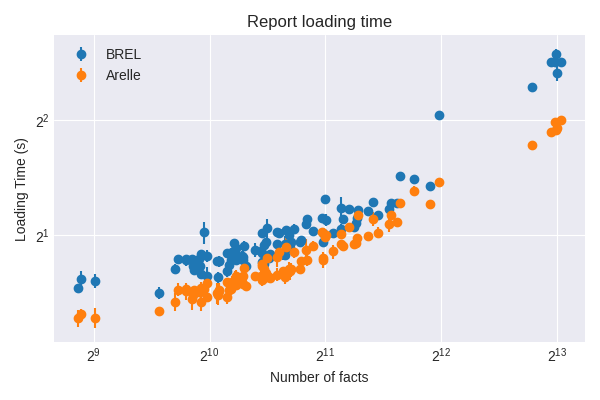
\includegraphics[width=\textwidth]{images/performance_graph.png}
    \caption{Performance of Brel and Arelle}
    \label{fig:performance}
\end{figure}

% The performance test includes 97 reports, whereas each report is run 11 times for both Brel and Arelle
% \footnote{The 3 missing reports are from Thermo Fisher Scientific and The Walt Disney Company, which were not listed on the SEC website at the time of the performance test.}.
% On average, Arelle takes 18\% less time than Brel to load the same report.
% The average time it takes to load a report with Brel is 2.17 seconds, while Arelle takes 1.81 seconds.
The performance evaluation encompassed 97 reports, each tested 11 times using both Brel and Arelle\footnote{The 3 missing reports are from Thermo Fisher Scientific and The Walt Disney Company, which were not available on the SEC website during the performance test.}.
On average, Arelle demonstrates an 18.5\% faster loading time than Brel for the same reports.
Brel's average loading time for a report is 2.17 seconds, compared to Arelle's 1.81 seconds.

% The standard deviation of the loading times for both Brel and Arelle is 0.05 seconds.
% This means that the loading times of both Brel and Arelle are consistent across different runs.
% The standard deviation of the loading times is also consistent across different reports with a few exceptions.
% These exceptions can most likely be attributed to the machine's background processes and are not significant enough to affect the overall performance of Brel and Arelle.
Both Brel and Arelle exhibit a standard deviation in loading times of 0.05 seconds.
This consistency in loading times is evident across different runs for both tools.
The standard deviation remains constant across various reports, with a few exceptions.
These outliers are likely due to background processes on the machine and do not significantly impact Brel's or Arelle's overall performance.
% The loading time difference between Brel and Arelle is statistically significant\footnote{Based on a p-value of 0.05}.
Based on a p-value of 0.05, we can statistically confirm the significant difference in loading times between Brel and Arelle.

% \subsection{Discussion}

% The performance of Brel is satisfactory.
% However, the difference in loading times between Brel and Arelle is statistically significant
% \footnote{Assuming a p-value of 0.05}.

% From a qualitative perspective, the report loading times of both Brel and Arelle are acceptable,
% as they are significantly faster than the time it takes to download all files necessary to load the report.
% In general, the download time of the report is the bottleneck in the process of loading an XBRL report.
% Downloading a report tends to be in the order of tens of seconds, while loading the report is in the order of seconds.
% This discussion on download times is deliberately kept vague, as download times are highly dependent on the user's internet connection and the size of the report.

From a qualitative standpoint, the loading times for both Brel and Arelle are acceptable,
being significantly shorter than the time required to download the necessary files for report loading.
% Typically, the download phase is the more time-consuming aspect of loading an XBRL report.
Typically, the download phase more significantly impacts the loading process of an XBRL report.
While download durations often span tens of seconds, loading times are generally within a few seconds.
The discussion of download times is intentionally kept vague, as these times vary greatly depending on the user's internet speed and the report's size.


\section{Results Summary}
Given the results of the evaluation, we can conclude that Brel is a robust and accurate tool for working with XBRL reports.
The Brel API is easy to use and provides a high-level interface for working with XBRL reports.
The performance of Brel is satisfactory.
Compared to Arelle, Brel is slower in loading and extracting data from XBRL reports.

The next chapter will discuss the conclusions drawn from the results of the evaluation and the future work that can be done to improve Brel.
